\documentclass[conference, compsoc]{IEEEtran}
%\documentclass[letter,11pt]{article}
%\documentclass[letter,10pt]{scrartcl}

\usepackage[utf8]{inputenc}
\usepackage[pass,letterpaper]{geometry}
\usepackage{graphicx}
\usepackage{listings}
\usepackage{color}
\usepackage{float}
\usepackage{bigfoot}
%\usepackage[square,sort,comma,numbers]{natbib}
%\usepackage{titling}
%\usepackage{mathtools}
\usepackage{helvet}
\usepackage{algorithmicx}
\usepackage{algpseudocode}
\usepackage{tabularx,ragged2e,booktabs,caption}

\ifCLASSOPTIONcompsoc
  % IEEE Computer Society needs nocompress option
  % requires cite.sty v4.0 or later (November 2003)
  \usepackage[nocompress]{cite}
\else
  % normal IEEE
  \usepackage{cite}
\fi


\setlength{\parindent}{0cm}



\pdfinfo{%
  /Title    (OpenMemDB: A Wait-Free, In-Memory Database)
  /Author   (Mike McGee, Neil Moore, Robert Medina, Jason Stavrinaky)
  /Creator  ()
  /Producer ()
  /Subject  ()
  /Keywords ()
}

\let\oldReturn\Return
\renewcommand{\Return}{\State\oldReturn}

\newcommand{\CC}{C\nolinebreak\hspace{-.05em}\raisebox{.4ex}{\tiny\bf +}\nolinebreak\hspace{-.10em}\raisebox{.4ex}{\tiny\bf +}}


\definecolor{codegreen}{rgb}{0,0.6,0}
\definecolor{codered}{rgb}{0.6,0,0}
\definecolor{codegrey}{gray}{0.9}

\newcommand{\inlinecode}[1]{\colorbox{codegrey}{\lstinline[language=C++]{#1}}}

\begin{document}

\title{OpenMemDB: A Wait-Free, In-Memory Database\thanks{Sponsor: Dr. Damian Dechev}}
\author{
\IEEEauthorblockN{Michael McGee} \and 
\IEEEauthorblockN{Robert Medina} \and 
\IEEEauthorblockN{Neil Moore} \and 
\IEEEauthorblockN{Jason Stavrinaky}
}

\date{2/1/2016}

\pagenumbering{gobble}
\maketitle
\newpage

\pagenumbering{arabic}
\begin{abstract}
OpenMemDB is an in-memory database that is implemented solely using wait-free
data structures. OpenMemDB is the first and only database currently developed in such a
way. OpenMemDB also provides linearizable correctness guarantees for all operations
executed on the database. OpenMemDB uses a form of snapshot isolation to ensure 
linearizability, and avoids the write-skew problem that can occur when using
snapshot isolation by eliminating writes that are out of data. 
OpenMemDB's biggest contribution is its completely wait-free 
implementation. Every operation executed in OpenMemDB is guaranteed to be wait-free 
and linearizeably correct. This implementation also scales competitively when compared 
against similar in-memory database management systems.
OpenMemDB achieves its best scaling in select heavy operation loads with nearly 
12 times speedup at 16 threads. This is better scaling than either VoltDB or MemSQL showed
in our testing. 
\end{abstract}

\section{Introduction}
While hard drives are getting faster due to the introduction of NAND flash-based drives,
they are still relatively slow when compared to main memory. Meanwhile main memory is 
following a long running pattern where it has precipitously dropped in price from costing 
thousands of dollars for a few megabytes to about \$40 for 8 gigabytes \cite{jcmit}. 
With this trend, we can take advantage and design fast databases that reside entirely in main memory. While the largest of datasets are still too large for main memory, 
some datasets are finally able to fit into main memory in modern systems due to the 
cheapness and advancement of memory module technology. 
\par\vspace{\baselineskip}
Most technologies have advanced 
along with hardware, however database management systems have struggled to improve
at a similar rate. This is mostly due to concurrency issues. Databases spend more than 30\% 
of execution time in synchronization-related operations, even when only running a single
client thread\cite{soares2015database}. And in this era, where a powerful server
can have more than a terabyte of RAM and well over 64 cores, effectively utilizing all of 
this processing power is essential. 
\par\vspace{\baselineskip}
Our approach, OpenMemDB, solves this problem by implementing a data-store 
using only wait-free data structures that scale extremely well with added cores. 
OpenMemDB is a SQL database designed from the ground up to provide fast access to shared
data without using any locks. This is achieved through the use of wait-free
data-structures provided by Tervel, a library of wait-free and lock-free data-structures
developed by Feldman et. al\cite{tervel:hazard_pointer}\cite{tervel:hash_map}\cite{tervel:vector}. The lack of contention on locks and the wait-free
guarantees that the Tervel data-structures provide will achieve the performance gains that 
have been lacking in the DBMS field. 
\par\vspace{\baselineskip}
OpenMemDB's biggest contribution is in being the first completely wait-free database 
management system. Wait-freedom is a progress guarantee for concurrent data-structures 
which states that all threads running operations on the data-structure are guaranteed 
to complete in a finite number of steps. This sort of guarantee can be vital in 
real-time systems where a hard limit needs to be placed on how long an operation 
is allowed to take. One situation in which OpenMemDB would be ideal is for use in real-time 
database systems, where data has a temporal validity, and all calculations using this data 
must complete within this valid range of time. An example of a real-time database system 
is a stock market analysis database. A database that is used to track the current state
of the stock market and run calculations based on the temporarily valid data. 
\par\vspace{\baselineskip}
OpenMemDB
is also well suited for any situation in which a large amount of calculations need to be 
executed on a relatively centralized data-set. This is due to the fact that OpenMemDB 
provides all threads access to every part of the database. Some database systems attempt to 
use data partitioning to help parallelize their operations, these systems would not be a 
good choice if the data-set could not be efficiently partitioned. OpenMemDB does not do any 
partitioning and still manages to achieve 90\% scaling at 8 threads and 60\% scaling at 32 
threads. 
\par\vspace{\baselineskip}
OpenMemDB also 
retains all necessary ACID properties, which is vital for most database systems. 
The requirements of being wait-free dictate that 
OpenMemDB is an in-memory database and thus avoids the bottlenecks associated with 
going to hard disk. OpenMemDB is written in \CC 11 and uses the modern constructs defined by 
that standard extensively.
\par\vspace{\baselineskip}

\section{Related Work}
There are several other in-memory database management systems that attempt to solve the 
problem of data-contention. This being the main source of slow downs for in-memory systems.

The database management system most related to OpenMemDB is MemSQL.
MemSQL uses lock-free data structures for every component of their database management
system. MemSQL uses lock-free skips lists and hash tables for the bulk of their data-store\cite{MemSQL}.
They also use MVCC (Multi-version Concurrency Control) to provide fast transactions. 
OpenMemDB does something similar with snapshot isolation. MemSQL also compiles SQL
statement to C++ code and stores this code to be used if the SQL statement is ever called
again. Something that OpenMemDB does not implement.

VoltDB is an in-memory database management system that uses pure SQL, is completely ACID
compliant, and does not use locks. They claim to achieve 100 times the performance of 
a traditional relation database management system, with near linear scaling with added nodes \cite{voltdb2010voltdb}. They claim to achieve 560,000 transaction per second on a 12
partition set up. 
VoltDB uses a shared nothing architecture. Their execution engine is single threaded, 
avoiding the overhead of locking or latching \cite{voltdb2010voltdb}. This requires
intelligent partitioning of data and does not allow for multi-threaded execution 
on a single partition. 

Silo is an in-memory database that uses optimistic concurrency control (OCC) to try and 
limit the affects of locks on their system. Silo avoids locking during the computation
of a transaction and waits until commit time to execute all writes to shared memory.
This avoids the contention involved in acquiring a lock until a short period of time 
at the end of transaction. This style of system can be particularly effective if
concurrent writes to shared memory are uncommon. Silo claims to achieve 700,000
transaction per second an a 32 core machine. Silo relies heavily on concurrent 
B+ tree for its back end data-store \cite{tu2013speedy}. 

Hekaton is Microsoft's main memory optimized database engine.
Hekaton uses a combination of lock-free data-structures and optimistic concurrency control
in order to achieve scaleable performance gains. Hekaton is like Silo and OpenMemDB in that 
it does not use partitioning to achieve performance gains. Any thread can access any 
row in a table without acquiring a lock\cite{diaconu2013hekaton}. Hekaton claims to gain
an order of magnitude performance gain over standards SQL Server\cite{diaconu2013hekaton}

%TODO fix the rest of this
%MemSQL\footnote{MemSQL can be configured as a Columnstore that stores data on disk.}
%and VoltDB are both fully in-memory DBMS as is OpenMemDB. This is where the
%similarities end as far as OpenMemDB is concerned. MemSQL and VoltDB on the other 
%hand both use distributed systems to achieve performance gains and they both differ from 
%OpenMemDB in a few ways. MemSQL uses lock-free data structures
%to store data and stores pre-compiled commonly used queries\cite{MemSQL}.
%VoltDB tries to make its performance gains by what they call Concurreny through
%scheduling\cite{VoltDB}. This is the process of using a single-threaded pipeline 
%that performs the task it was scheduled. This limits the need for locking during
%transactions by intelligently scheduling the transactions so that locks are not
%necessary. This approach eliminates the time spent obtaining and updating a lock
%but limits parallelization. There can not be true concurrent access on shared data. If 
%there are a number of operations that need to be executed on the same table in a database; 
%these operations will be scheduled sequentially. The only parallelism that occurs is during
%operations on unrelated data. Our approach allows for concurrent operations to take place
%no matter what data is being accessed.

\section{Technical Approach}
Our database is built upon wait-free data structures found in Tervel, a collection of
lock-free and wait-free data structures created by Feldman et al\cite{tervel:hazard_pointer}\cite{tervel:hash_map}\cite{tervel:vector}. 
We use the common definition of wait-freedom as found in Herlihy's definitive text, which
states that all threads must make progress within a finite amount of time\cite{herlihy:waitfree}. OpenMemDB is 
built to be wait-free and linearizable by utilizing Tervel data structures to create the 
underlying data structures used by the database to service queries and commands.

OpenMemDB tables are made up of a composition of Tervel data structures, namely the hash map and the
vector. The hashmap handles the relation of a table's name to its table object. The vectors used in a
way that a vector, referred to as the table vector, holds references to other Tervel vectors that contain
the actual data used. As only references to records are stored in the table vector, most operations on the
table take place as whole record operations rather than a more fine-grained approach that would update
records on a per-column basis.

The datastore uses snapshot isolation to increase read performance and minimize the amount of time accessing
the shared data structures. Snapshot isolation is the technique where a thread or transaction copies the data
locally and then manipulates it, which avoids performing those manipulations directly on the data structures.
A side effect of snapshot isolation is write skew, which occurs when a write operation takes place even though the
predicate that determined that record should be written to is no longer valid.
We avoid write skew caused by snapshot isolation by only committing the writes
if the expected data is in the table. This is done by using the Compare and Swap(CAS) operation provided
by Tervel's vector data structure. The CAS operation checks if the element in the vector is the
expected value and swaps the value with the given value if that check succeeds. Tervel's CAS
operation is wait-free and atomic, so any contention will have a clear ``winner'' or ``loser'' in terms
of if a thread succeeds in updating or writing to the vector. This translates to a thread failing to update the
table with the new record reference if another thread replaces the record before the attempted write but 
after the initial read of the record.  The loser thread or threads then report that they encountered 
contention during execution, but continue to perform their operation as best as possible.

\section{Experimental Results}
Our experiments took place on a 64-core AMD Opteron system with 300 GB of system memory running Ubuntu 14.04 and 
GCC 4.8.4. Each database was given the same series of operations to perform for each test, with each database 
connected to locally so as to remove network latency from the test. We explicitly only tested other databases
with SQL frontends, as our goal was a SQL database. We tested various workloads in order to evaluate 
the databases' ability to interleave writes and reads at the same time as well as particularly write-heavy 
loads. Each test was run with 1, 2, 4, 8, 16, 32, and 64 cores available to the database which maximizes the amount of hardware processors
available to the OS but does not exceed it. 
\par\vspace{\baselineskip}
We ran three tests on all of the databases: an insert only test, a select only test, and
a mixed test that consisted of 33\% writes and 66\% reads.
The resultant scaling found by running these tests can be seen in the tables below. 

\par\vspace{\baselineskip}
\begin{figure}[H]
\begin{center}
\captionof{table}{OpenMemDB Scaling} \label{tab:omdbScaling}
  \begin{tabular}{  l  l  l  l }
    \midrule
    \bf Threads & \bf Insert & \bf Select & \bf Mixed \\ \midrule
     2 & 1.84 & 1.93 & 1.94 \\ \midrule
     4 & 2.94 & 3.08 & 3.54 \\ \midrule
     8 & 4.19 & 6.97 & 7.33 \\ \midrule
     16 & 4.98 & 11.87 & 13.10 \\ \midrule
     32 & 4.75 & 19.05 & 20.44 \\ \midrule
     64 & 3.16 & 26.03 & 27.25 \\ \midrule
  \end{tabular}
\end{center}
\end{figure}

\par\vspace{\baselineskip}
\begin{figure}[H]
\begin{center}
\captionof{table}{MemSQL Scaling} \label{tab:memsqlScaling}
  \begin{tabular}{  l  l  l  l }
    \midrule
    \bf Threads & \bf Insert & \bf Select & \bf Mixed \\ \midrule
     2 & 1.20 & 1.58 & 1.68 \\ \midrule
     4 & 2.31 & 2.62 & 3.31 \\ \midrule
     8 & 4.53 & 3.74 & 5.63 \\ \midrule
     16 & 8.54 & 4.85 & 10.80 \\ \midrule
     32 & 15.13 & 4.87 & 18.21 \\ \midrule
     64 & 20.18 & 1.80 & 10.30 \\ \midrule
  \end{tabular}
\end{center}
\end{figure}

\par\vspace{\baselineskip}
\begin{figure}[H]
\begin{center}
\captionof{table}{VoltDB Scaling} \label{tab:voltScaling}
  \begin{tabular}{  l  l  l  l }
    \midrule
    \bf Threads & \bf Insert & \bf Select & \bf Mixed \\ \midrule
     2 & 1.75 & 1.61 & 1.42 \\ \midrule
     4 & 3.58 & 2.70 & 2.83 \\ \midrule
     8 & 6.13 & 4.51 & 3.93 \\ \midrule
     16 & 9.12 & 7.97 & 5.98 \\ \midrule
     32 & 10.71 & 11.92 & 7.12 \\ \midrule
     64 & 10.56 & 15.30 & 7.27 \\ \midrule
  \end{tabular}
\end{center}
\end{figure}


Table~\ref{tab:omdbScaling} shows the scaling achieved by OpenMemDB for each of the three
benchmarks that were run. As is clear OpenMemDB scales much better in select only tests. 
MemSQL has the best select only scaling of all of the databases that were bench-marked.  
Table~\ref{tab:memsqlScaling} shows the scaling for MemSQL for each of the three benchmarks. 
MemSQL does not scale as well as OpenMemDB in write heavy tests, this could be due to a number of factors
and further testing is needed to assess the cause.
Table~\ref{tab:voltScaling} shows the scaling for VoltDB for all three benchmarks.

\begin{figure}[H]
 \begin{center}
   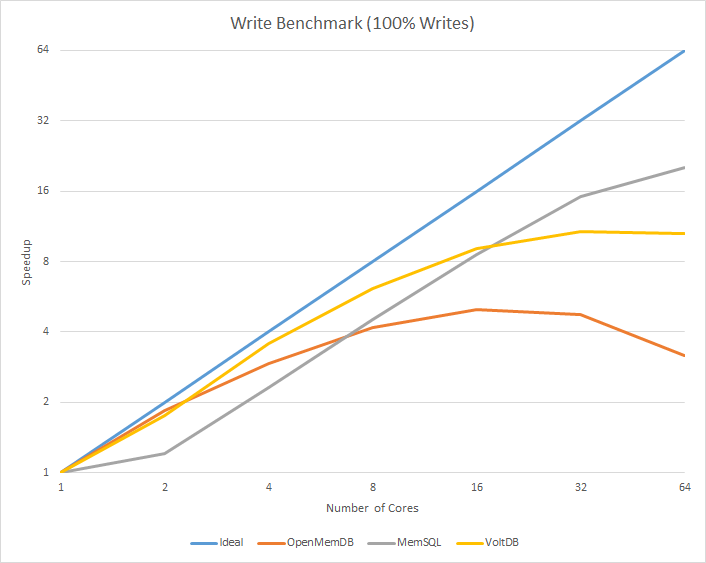
\includegraphics[scale=.5]{WriteBenchmark.png}
  \caption{500,000 writes on the selected databases}
  \label{fig:writeBenchmark}
   \end{center}
\end{figure}

\begin{figure}[H]
   \begin{center}
   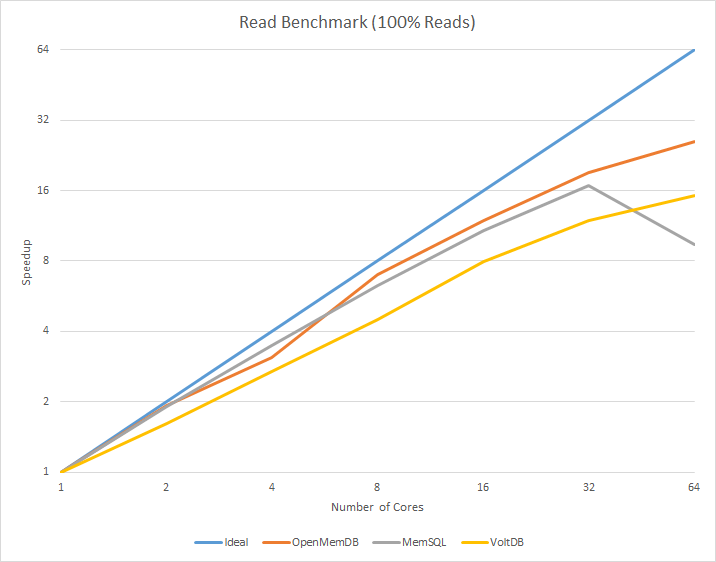
\includegraphics[scale=.5]{ReadBenchmark.png}
  \caption{10,000 reads on the selected databases}
  \label{fig:readBenchmark}
   \end{center}
\end{figure}

\begin{figure}[H]
 \begin{center}
   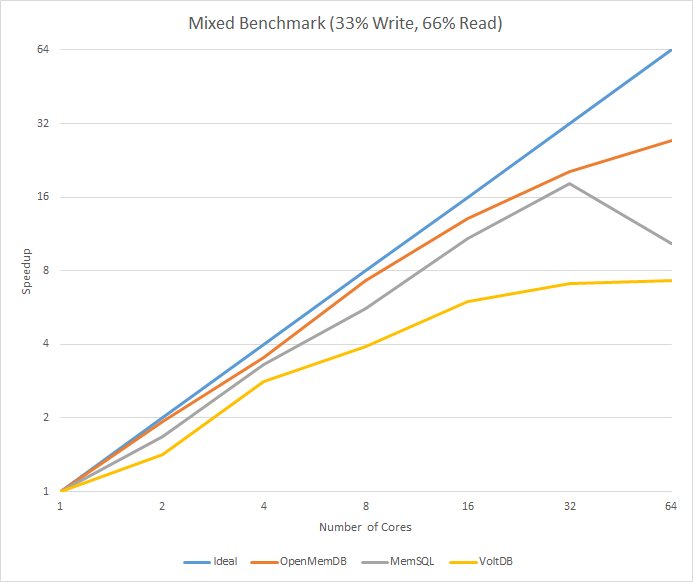
\includegraphics[scale=.5]{MixedBenchmark.png}
  \caption{10,000 mixed reads and writes on the selected databases}
  \label{fig:mixedBenchmark}
   \end{center}
\end{figure}

\section{Conclusions}
We have presented OpenMemDB, an in-memory and wait-free database that achieves competitive scaling when compared to other
in-memory SQL database management system.  OpenMemDB scales particularly well with read heavy workloads, achieving 90\% 
scaling at 8 threads and 60\% scaling at 32 threads when running our select bench-mark. OpenMemDB is the first, and only fully
wait-free database in existence at the time of writing this paper. 
\par\vspace{\baselineskip}
Based on the encouraging scaling achieved, further work toimprove individual thread performance would bring this database
closer to commercial viability, in particular with embedded systems where consistent latency is preferable to inconsistent
performance. 
\par\vspace{\baselineskip}
Some of the areas that can be improved with more time would be: improving the memory allocation model to reduce thread
synchronization, further optimizations of the tokenization and parsing of SQL statements, improved support for standard
SQL operations and data types.

\newpage
\bibliography{WorkshopPaper}
\bibliographystyle{acm}
\newpage

\end{document}
